\documentclass[11pt,a4paper]{report}
\usepackage[utf8]{inputenc}
\usepackage{graphicx}
\usepackage[acronym,footnote,description]{glossaries}
\usepackage{listings}
\usepackage[parfill]{parskip}
\usepackage{natbib}
\graphicspath{ {images/} }

\makeglossaries

\makeatletter
\defglsdisplayfirst[\acronymtype]{%
  \firstacronymfont{#1}#4%
    \protect\footnote{%
      \glslink[\@gls@link@opts]{\@gls@link@label}{#3}: #2}}%
\makeatother

\author{H\aa vard A. Heggheim\\[1cm]
Supervisors: Lars Petter Helland \&\\ Anders Øvreseth}
\date{\today}

\title{\vspace{-4cm}{
 {\huge Interworking WebRTC with Enterprise Multimedia Communications}\\[0.4cm]
 {\large Bergen University College and University of Bergen}\\
 {\large Joint Master's Programme in Software Engineering}\\[1cm]
 {\vspace{+5cm}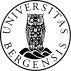
\includegraphics[height=3cm]{uiblogo.png}}
 {
\includegraphics[height=3cm]{hib_small.jpg}}
 \vspace{+4cm}
}}


\begin{document}


% TITLE %
\maketitle


% PRE SECTION %
\chapter*{Abstract}
%!TEX root = ../main.tex

page 211
state research problem
announce key themes
state the main point or launching point that anticipates the main point

context+problem+main point

put in key search words

\begin{abstract}
% The use of communication technologies today consume a large time of our daily lives. A lot of these technologies are now moving to Internet based solutions. Some of these services are collaboration tools that do video/audio and application sharing. This thesis will look at streaming media on the web in a collaborative enterprise environment. There are currently many Internet based communication services existing today that does this, but most of these are not open, cost money and require the installation of a plugin. This thesis will look at how Visual Solutions can integrate the new WebRTC APIs for doing real-time streaming of media in the browser with their current visual collaboration solution Virtual Arena.

% The aim of this thesis is to find the most suitable way for Visual Solutions to implement live media sharing in the web browser with their current application Virtual Arena. The goal is to detect challenges and problems that might occur with the use of the new Web APIs.

% The HTML5 standard introduces many new APIs that give web browsers the ability to communicate directly with each other in real-time. But there are many solutions and the different providers doesn't seem to agree on a single solution. This thesis will examine using these new APIs to see how we can integrate the browser in current media collaboration systems. The goal being to determine the feasability of using these new APIs and evaluate their usage. This thesis hopes to aid in developing solutions for media sharing in the browser that can be used in an enterprise setting.
\end{abstract}


This is a study on how to integrate \gls{rtcweb} with a enterprise communication system. Each system is broken down into several components on the transport level. A gateway model interoperating between the two architectures are created and then evaluated by looking at similar systems.

\\gls{rtcweb} is defined as the underlying technologies of a set of APIs drafted by the \gls{w3c} as \gls{webrtc}. It supports browser-to-browser applications for audio/video chatting without plugins. \gls{wrtc} is currently seeing great support with two of the major browser vendors; namely Google and Mozilla. Both Apple and Microsoft currently lag a bit behind, but they are both active in the working groups that define the standards. A ton of new companies are appearing using this new technology because of the easy entry these APIs provide. The browser APIs are simple to use and let's you basically create your own phone company over a weekend. This has turned the eye of bigger telecom vendors like Cisco and Ericsson. All of them are looking into how they can use \gls{wrtc} in the future. One of the greatest advantage of utilizing \gls{wrtc},% is the whole range of new devices you suddenly have access to. Using the optimized audio and video engine of \gls{rtcweb}, you can scale for pretty much any device that has support for the latest Chrome or Firefox browser. The integration of \gls{wrtc} allows for easier adopting of the \gls{byod} to work policy that permits employees to bring their personally owned mobile devices (laptops, tablets, and smart phones) to work. The problems of using a mobile \gls{wrtc} client within an enterprise setting is discussed in this thesis.  

Using guidelines derived from looking at different ways of doing this integration, in order to aid in deciding if this is a feasible way to go about getting support for mobile devices in current enterprise systems. The use of a gateway outlined in this thesis is the main topic together with recommendations for implementing a mobile \gls{wrtc} client for tablets and smartphones.

\tableofcontents

\chapter*{List of Figures}
%\input{chapters/figures}%

\chapter*{Acronyms}
%!TEX root = ../main.tex

\newacronym[description={defines a standard packet format for delivering audio and video over IP networks.}]{rtp}{RTP}{Real Time Protocol}
\newacronym[description={develops and promotes Internet standards.}]{ietf}{IETF}{Internet Engineering Task Force}
\newacronym[description={}]{http}{HTTP}{Hypertext Transfer Protocol}
\newacronym[description={}]{https}{HTTPS}{Hypertext Transfer Protocol Secure}
\newacronym[description={}]{w3c}{W3C}{World Wide Web Consortium}
\newacronym[description={}]{ssrc}{SSRC}{Secure Real-time Transport Protocol}
\newacronym[description={}]{mcu}{MCU}{Media Control Unit}
\newacronym[description={}]{udp}{UDP}{User Datagram Protocol}
\newacronym[description={RFC 4566}]{sdp}{SDP}{Session Description Protocol}
\newacronym[description={RFC 5389}]{stun}{STUN}{Session Traversal Utilities for NAT}
\newacronym[description={RFC 5766}]{turn}{TURN}{Traversal Using Relays around NAT}
\newacronym[description={}]{nat}{NAT}{Network Address Translator}
\newacronym[description={RFC 6347}]{dtls}{DTLS}{Datagram Transport Layer Security}
\newacronym[description={RFC 4960}]{sctp}{SCTP}{Stream Control Transport Protocol}
\newacronym[description={RFC 3711}]{srtp}{SRTP}{Secure Real-time Protocol}
\newacronym[description={RFC 5245}]{ice}{ICE}{Interactive Connectivity Establishment}
\newacronym[description={http://www.w3.org/TR/webrtc/}]{wrtc}{WebRTC}{Web Real-Time Communication}
\newacronym[description={Specifies how some software components should interact with each other}]{api}{API}{Application Programming Interface}
\newacronym[description={Integrated communication medium based on the upcoming W3C standard WebRTC}]{rtc}{RTC}{Real-time communication}
\newacronym[description={http://tools.ietf.org/html/draft-ietf-rtcweb-jsep-03}]{jsep}{JSEP}{JavaScript Session Establishment Protocol}
\newacronym[description={https://tools.ietf.org/wg/rtcweb/}]{rtcweb}{RTCWEB}{Web Real-Time Communications}



% MAIN SECTION %
\chapter{Introduction}
%We live in a world where communication plays a major role in how we conduct business. Location independant work roles are more common now than ever before. Two persons no longer have to sit next to each other in order to collaborate on a project, they just need good real-time communication tools. There are several methods of doing communication, including: web-based communication, video conferencing, e-mails, telephoned meetings and forum boards. In may 2011, Google released an open-source project for browser-based real-time communication known as \gls{wrtc}\cite{google-release-of-webrtc}. There is an ongoing effort to standardise this work. The term \gls{wrtc} is usually used in general to cover all aspects of this technology, however specifically the underlying protocols and codecs are defined as \gls{rtcweb} and is standardised by the IETF\cite{ietf}. \gls{wrtc} actually only covers the browser APIs defined by the W3C\cite{w3c}. These APIs are integrated directly in the browser and allows smaller enterprises to create advanced communication applications in a much simpler way than ever before. These new APIs has the advantage of being able to work on every single device that runs a \gls{wrtc} compatible web browser. By integrating \gls{rtcweb} into older communication systems, we allow these systems to interact with a whole range of new devices. By modeling a bridge between \gls{wrtc} and enterprise communication systems, we can reach these devices without having to modify or break current system architecture.

Large companies like Cisco and Microsoft are big players in the communications industry. They sell tools that makes us able to communicate in real-time. These tools are expensive and generate a lot of revenue for these companies, but now we see a rise of smaller enterprises taking market shares in certain areas from these big companies. These enterprises are efficient at using new technologies that simplifies greatly the way we can develop communication applications. \gls{wrtc} is one of these new technologies. It is directly integrated in the web browser, so that we can use simple web APIs to handle communication between peers. All the advanced underlying technologies of doing transportation of media, routing the traffic through firewalls, and dynamically adjusting bandwidth usage, is taken care of by the browser. Using these new simple APIs we can quickly develop advanced communication systems, and since they are integrated directly in the browser, it is also possible to get mobile device support with a lot less effort than before. The main problem here is that this technology does not have any way of communicating with older communication systems. This is a problem for companies that want to take advantage of the new possibilites this technology provides, such as mobile support for almost all platforms that can run a web browser.

In collaboration with the company Visual Solutions\footnote{http://www.bbvisuals.com/} I will look at how we can integrate an older communication system with the new \gls{wrtc} technology. This work could be of benefit to all communication companies that want's to take advantage of the new possibilities that \gls{wrtc} provides. Visualize yourself getting late to a meeting, with a simple click on a link you got in an invitation, you will be able to participate in the meeting from your mobile device, wherever you are with an internet connection, this would be possible. Visual Solutions have created an application called Virtual Arena that does collaboration between peers thorugh sharing of audio, video, and applications. This application will be used as a reference of a typical enterprise communication system.

This thesis will model a solution to bridge \gls{wrtc} with a typical enterprise desktop communication system. I do this by going through all the tehnologies that \gls{wrtc} requires to be implemented for a connection between two peers to occur. Looking at different ways of creating a gateway between two systems, I will suggest an architecture with all the components required for making the interaction. I will also focus especially on the communication between mobile devices, as this is one of biggest advantages of utilizing \gls{wrtc}.

This thesis will begin by giving an introduction to \gls{wrtc} and basic transportation protocols. To understand how \gls{wrtc} works you need to understand a lot of new concepts. These will be described in the background chapter. Then I will describe in detail what the main problems of bridging \gls{wrtc} with a desktop enterprise communication system are. I will then model a gateway that makes communication between \gls{wrtc} and Virtual Arena possible. I will also look at different problems that needs to be handled when developing a mobile \gls{wrtc} client. Lastly I will take a look into the future and make a prediction of what new features will soon be available for \gls{wrtc}.%

\chapter{Background}
%%!TEX root = ../main.tex

This chapter will look at current video collaboration solutions and solutions that have tried video streaming utilizing P2P technology.

\section{State of Collaboration Today}
There exists millions of SIP and RTP devices that are used in Enterprises. These devices does not have a common set of features. Some are upgradeable, some are not. These devices include PBXs, desk-phones, soft-phones, PRI gateways, and voicemail servers. Some SIP devices implement ICE, while others do not even generate RTP and only support older protocols. Several software-based SIP agents (softphones) implement ICE, but almost no
PSTN gateways or PBXs do. And very few media servers do.
\\

Huge vendors in the communications business like Cisco, Polycom and Huawei initially based their business on hardware systems, but customers are now migrating over to software-based solutions and lower-cost systems. This trend is allowing new companies to come up with alternate solutions.
\\
It is difficult to require businesses to upgrade all their devices in order to communicate with WebRTC-enabled Browsers. Therefore we need an interworking function to make the systems work together. An interworking function may be needed, but it is essential to minimize the cost of such a function, or not need one to begin with. 
\\

\subsection{Security}
Another problem by utilizing the Internet and third party providers is security. The Javascript in Browser cannot be fully trusted. The current solution is to require a peer to use ICE using STUN for connectivity checks. A WebRTC browser cannot allow session media to be used unless peer uses ICE. Since many SIP devices does not support ICE, and will not be upgraded, an interworking device is needed.
\\
These kinds of problems, hinder innovation and we often end up using old legacy systems. Thankfully the next generation of tech leaders is realizing that using video makes them more productive, it helps reduce cost and plays a role in attracting the best talent available. We will see video collaboration tools on the rise in the upcoming years.


\section{Peer-to-peer technology use in the enterprise}

\subsection{Skype}
Skype utilizes P2P by leveraging all of the available resources in a network, this is probably why they can manage free communications. Using centralized resources is very costly.
Even the user directory is decentralized. While Skype has very successfully developed a video collaborations system utilizing P2P technology. The quality depends on the users available resources. A server would have resources dedicated and finetuned to this kind of communication.

\subsection{BitTorrent}
Livestream are great but they tend to go down if a lot of people wants to watch the stream at the same time. The idea is the same as with Skype., but the technology is built on top of the BitTorrent protocol. It chops up the feeds and distributes among a bunch of peers. This cuts down on lag and latency.
 utlilizes	

\subsection{Flash}
Codename Cirrus enables peer assisted netoworking using the Real Time Media Flow Protocol within the Adobe Flash Platform. Flash is the most used technology today for serving video content. YouTube Live tech?

\subsection{Silverlight}
netflix

\subsection{MCU}
A multipoint control unit (MCU) is a device used to bridge videoconferencing connections. The multipoint control unit is an endpoint on that provide the capability for three or more peers to participate in  a conference by combining streams into a singular one.
BB Visuals uses MCU!!

\section{Browser based solutions}

\subsection{Hangout}
Google+ Hangouts is an instant messaging and video platform developed by Google. It allows users to hold conversations between two or more users. The service can accessed through Google+ or through mobile apps. But the service uses a proprietary protocol developed by Vidyo, so there are for example, no free software clients for Google+ Hangouts.

\subsection{FaceTime}
FaceTime is a video telephony software application developed by Apple for the Iphone and iOS Macintosh computers. You can activate FaceTime when during a telephone call by pressing the FaceTime button. FaceTime is based on open standards:
H.264, SIP, STUN, TURN and ICE, RTP and SRTP. The service requires a client-side certificate. This protects against unauthorized access to the service controlled by Apple. This is why the service has not been implemented on other devices.
SIP ICE RTP SRTP

Vidyo Hangout FaceTime
\\
while video conferencing is the most common tool in video collaboration type services. Video collaboration can include screen-sharing, remote desktop, sharing 3d image screen, presenting, whiteboarding
\\
Nd native system. WebRTC is open-source, requires no-plugins, and allows.

\chapter{Industrial Case}
%!TEX root = ../main.tex

This thesis is written in cooperation with Visual Solutions\footnote{http://www.bbvisuals.com/}.

Visual Solutions is a Norwegian company in the BB Visual Group\footnote{http://www.bbvisualgroup.com/} Their primary business is within the integration of operations for the oil and gas industry. They have offices in Houston, US, Brighton, UK and a headquarter in Bergen, Norway.

Visual Solutions contribute tailor made solutions enabling and improving collaboration and cross-disciplinary interaction across organisation units and geographic locations.

One of their applications Virtual Arena\cite{solutions_b2|virtual_2014} is a powerful and interactive tool that allows IP-based application sharing within collaborative sessions. Virtual Arena supports one-to-one, one-to-many and many-to-many collaborative scenarios, with support for high-performance application sharing, audio and video communication from an advanced 3D shared scene.

\section{Visual Solution's vision}
In today's  world everybody owns some kind of mobile device. If a user could enter a collaborative session from the web browser of their own simple mobile device, this would be of great benefit to the customer. The user would not have to install any additonal plugins or software to their device. Many new API's are currently being developed to improve communication and hardware access in the web browsers. The \gls{w3c} has drafted a document that defines a set of API's to allow media to be sent to and from another browser or device implementing the appropriate set of real-time protocols.

Visual Solutions wants to investigate how far development has come with these new API's and if their vision can be accomplished by using them in their application.

The problem can be defined in two sub-problems:
\\
\\
\textbf{Problem 1}\\
Is it possible to use these new API's together with Visul Solutions current application? How can these new API's be implemented with their current software solution Virtual Arena?
\\
\\
\textbf{Problem 2}\\
It is in Visual Solutions interest to gain knowledge of how good the support for these new API's are today in desktop browsers and on mobile devices. This would give an indication to whether or not there is anything to gain from investing in further development.

\chapter{Problem Description}
%!TEX root = ../main.tex

This chapter will describe the problems of integrating \gls{wrtc} with enterprise communication systems. It will also present the goals of doing this research, present the research question, define the research and implementation method, then lastly present the expected results.

\section{Problem Description}
The \gls{byod} policy allows workers to bring their own mobile or tablet device to work. In enterprises this policy generates a lot of problems regarding how to handle security. One thing people need is to be able to access their enterprise internal communication system from their own device. The \gls{wrtc} technology allows us to easily create mobile clients, but how do we get these to interact with existing enterprise communication systems? We need some kind of technology that interworks these two technologies. What we need is to have the underlying protocols of \gls{wrtc} work together with traditional enterprise communication protocols. We also need to have the two systems being able to communicate with each other through message exchanging and signaling. Last but probably most important is how to handle access policies and crossing the enterprise firewall. The advantages of supporting \gls{rtcweb} in enterprise communication systems are huge. Immediately the system can access any WebRTC-enabled browser. This means we can reach out to a whole range of new devices. We basically get universal mobile support, easy client integration with top security, and no need to download applications or plugins, the app runs directly in the browser.

% Doing real-time communication in the web browser is nothing new, flash implementations have existed for a long time, and Google's Hangout is quite popular, but \gls{wrtc} seems to have some important advantages over the other technologies.

% \begin{itemize}
%     \item Universal mobile support
%     \item Easy integration, with a high focus on security.
%     \item No need to download clients or plugins.
% \end{itemize}

% By looking over the drafts done by \gls{w3c}, \gls{wrtc} seems to be well suited for doing collaboration directly in the web browser.


% \section{Problem statement}
% \gls{wrtc} seems to be the best solution for doing video conferencing on the web, and both desktop and mobile web browsers have some degree of support which improves on a nightly basis.

% While other solutions like Flash may have better support at the moment, there is a clear indication that the web is moving towards open standards\cite{jennings_real-time_2013}. A lot of effort is being put into \gls{wrtc} at the moment by big companies like Google and Mozilla to create this technology, however there are still disagreements about which audio/video codecs is going to be used\cite{philippe_video_2014}.

% All the browsers that support \gls{wrtc} only support different subsets of the features specified by the \gls{w3c}. Therefore a lot of experiments had to be conducted to see what kind of features worked and which did not. It was also necessary to test different codecs, to see which ones was allowed to use in the different browsers.

% It's interesting to see if this technology is mature and usable enough to work in a enterprise environment. We also have to see what features are planned for the future of \gls{wrtc}, and if support for more platforms are coming.

\section{Research question}
This thesis will try to answer the following question:
\\
\\
\textbf{How can we best integrate \gls{wrtc} with a enterprise communication system for doing collaboration?}
\\
\\
Supporting questions:

\begin{itemize}
    \item How should we approach developing a \gls{wrtc} client for mobile devices?
    \item How will this technology improve in the near future?
\end{itemize}

By answering these questions, it will be possible for multiple businesses to take advantage of the \gls{wrtc} technology by utilizing a gateway that interoperates with their existing systems for doing communication, with the addition of some important notes on developing clients for mobile devices.

\section{Research method}
The research method used in this thesis, is a quantitative experimental method, using systematic investigation and analysis of the different implementations in browsers of the drafted APIs by the \gls{w3c}. Experiments is done to examine the actual workings of the implementations to uncover support for the protocols and codecs defned in \gls{rtcweb} by the IETF. Practical experiments are run in Chrome, Firefox, and Chrome for Android. Different SIP applications will be used to test interoperation through a gateway. Wireshark\footnote{Wireshark is a network protocol analyzer} is used to capture and analyse traffic to see what type of data is being transmitted. An open source \gls{wrtc} gateway is tested to see how well it interworks with \gls{wrtc} and other systems. 

\section{Implementation method}
A model is created to reuse as much of existing architecture as possible from the enterprise communication system. This is done to separate components as much as possible from the existing system, and thus this work extends beyond the specific industrial case in this thesis. The specifics of the industrial case will be explained further in the next chapter.



% \section{Existing work}
% There exist's a lot of tutorials on creating very simple implementations of \gls{wrtc} on the client side, usually setting up one-to-one connections using a third-party service for doing signaling. More advanced guides shows how you can setup your own server to do signaling using WebSockets\footnote{WebSocket is a protocol providing full-duplex communications channels over a single TCP connection}.

% This is great, but to be able to create an advanced server that acts like a gateway between \gls{wrtc} and Virtual Arena, we need to look further. Looking at commercial solutions that could potentially be of some help, most of them are closed. But there is one open source project named webrtc2sip\cite{doubango_telecom_webrtc2sip_2014} which acts like a gateway between \gls{wrtc} and \gls{sip} to allow a browser to create and receive calls from a legacy \gls{sip} network. It's written in C++ and it's open source, but not very well documented. It also doesn't offer exactly what we need, as it is designed to work with \gls{sip} systems. An other interesting project is an open-source \gls{mcu} called Licode\cite{lynckia_licode_2014}, this one is not designed to include external \gls{rtp} streams, but if this functionality could be implemented server side along with a proxy for doing signaling, it could be a very interesting project.

% There is no good service on the web that provides live data on how far the support has come on different browsers. There is one service that will check for WebRTC and WebSockets connectivity on \url{http://www.check-connectivity.com/}. There are blogs and articles that provide tables showing who has implemented which APIs, but most will be outdated.


\section{Expected results}

\begin{itemize}
    \item From this thesis I will have provided a model of how an enterprise can integrate WebRTC with their own communication systems. I want to provide information and guidelines about all the necessary technologies that needs to be implemented.
    \item Also I would like to provide guidelines on how to design a mobile friendly WebRTC client.
\end{itemize}


%\chapter{HTML5}
% %!TEX root = ../main.tex

This chapter gives an introduction to the new \gls{wrtc} APIs.

\gls{wrtc} is a collection of standards, protocols, and Javascript APIs. The combination of these enables web browsers to do peer-to-peer audio, video and data sharing between browsers. There is no plugin or third-party software required. Real-time communication is now becoming a standard feature in browsers that any web site can use via simple APIs.

Delivering such functionality such as live audio and video sharing and data exchange requires a lot of new processing capabilities in the browser. This is abstracted behind three primary APIs:

\begin{itemize}
\item MediaStream: capturing audio and video streams
\item RTCPeerConnection: communication of audio and video data
\item RTCDataChannel: communication of arbitrary application data






With HTML5 Video you can embed video into your web page, without the need for external plugins like Adobe Flash, Microsoft Silverlight or Apple Quicktime. It’s natively integrated into the browser, which allows for you to have full control over the element. The need to have video in web pages will be discussed also how we never before had a uniform implementation in all major browsers.

\section{History}
The <video> element was first mentioned in 2005, then the first browser rolled out a nightly build in November 2007. Before the introduction a web developer could include video only through  embed elements, which required browser plugins. Initially these plugins would launch an external video player that was installed on the users system. Later with the release of the Flash Player, Macromedia introduced video support into its browser plug-in. Flash later became the major plug-in for providing rich Internet Applications which led to many users having it installed on their system. It became the standard for publishing video online without having to encode in three different codecs. YouTube launched in May 2005, and it was natural for them to choose using Macromedia Flash. Adobe later bought Flash and was therefore known as Adobe Flash. The discussion continued on the <video> element and the need for a standard baseline encoding format. Apple refused to implement Flash on their mobile platforms simply because they would no support using closed platforms that are dependant on third parties. With the HTML5 open standards, developers will be able to have full control over all layers of web applications, including the DOM, CSS, and JavaScript. This includes the need for all major browser to implement a common standard.

\section{A Common Standard}
YouTube used Adobe Flash with MP4 H.264/AAC codecs. Choosing the same codecs as Adobe Flash would allow for a simple migration. But there has been many concerns around H.264 that it uses a lot of hardware resources, therefore not being ideal to run on mobile devices. The situation changed when Google announced the WebM project. A new open-source royalty-free video file format, which included the VP8 video codec together with the Vorbis audio codec placed inside a Matroska container. Google has worked hard to encourage using their format as the baseline standard. As of now the current implementation status is like this:

\section{TCP vs UDP}
what they are + differences

\section{Adaptive streaming}
Adaptive streaming is a core component of online video. It enables buffer control to reduce waste of bandwidth, fast seeking, quality adjustments and live streaming which is most important to this report. Currently only Apple’s platform support HTTP Live Streaming using the HLS protocol. But the W3C is working on developing MPEG-DASH standard and Media Source Extensions that will allow for custom adaptive streaming applications. Chrome supports this API today, with the others working on implementations. The specification will allow JavaScript to construct media streams independant of how the media is fetched.
Other proprietary technologies are Microsoft Smooth Streaming and Adobe HTTP Dynamic Streaming.
\\
MPEG-DASH is a fragmented HTTP streaming protocol. A single video file is divided into many discrete chunks of video/audio data. These fragments can then be loaded as needed by the player and fed into a video buffer using the HTML5 MediaSource Extensions.

\section{Streaming Using RTP/RTSP vs HTTP}
Streaming media differs from ordinary media by the fact that streaming media is played out (almost) as soon as it is received. The traditional way of delivering video over the internet is to wait for the entire video file to be downloaded. The reason for developing streaming services was to enable a sender to transmit live content.

A huge increase in network capacity has made streaming audio and video over the Internet feasible. There is a set of standardized protocols for streaming real-time media over computer networks defined by the \gls{ietf}. This section will discuss the abilities of these protocols. For this thesis RTP and HTTP are the most important protocols, almost all protocols are based on these, but with added security layers.

\subsection{RTP}
RTP, the Real Time Streaming Protocol is the most used today. There is a need for browsers to also support this protocol, but currently there is very limited support. Live streaming can also be achieved using HTTP or HTTPS using adaptive streaming technologies. A problem with RTP is that it requires connection on specific ports. The problem is that unless these specific ports are opened - the firewall will block traffic from them. RTP uses UDP which allows live connection, if the network gets congested, RTP will lose the data. But RTP can also be run over TCP, this would be almost the same as HTTP which uses TCP. You will not lose data, but there can be a delay in the stream. It is used in situations where live communication with low latency is required. Adobe Flash Media Server is very similar to RTP.

\subsubsection{WebRTC}
\ac is an effort in collaboration amongst the different web browser vendors to add real-time voice and video communication capabilities to browsers. These new standards will bring phone, TV and computer all on a common platform. It is based on \ac{udp} communication with \ac{srtp} on top with \ac{dtls} for security. The specification is divided in three \ac{API}s:

MediaStream(aka getUserMedia)
represents syncronized streams of media taken from the camera and microphone of a media device.

RTCPeerConnection
is the component that handles stable and efficient communication of streaming data between peers.

RTCDataChannel
specification is still under heavy development, but this will allow for \ac{p2p} exchange of arbitrary data, such as file transfer.

Signaling
\ac{webrtc} uses RTCPeerConnection to communicate streaming data between browsers, but also needs a mechanism to initialize and coordinate communication, a process known as signaling. Signaling protocols are not specified by \ac{webrtc}. Instead developers can choose whatever messaging protocol they prefer, such as \ac{sip} or \ac{xmpp}. So while one of the ideas of \ac{webrtc} was that the browser would be able to send information, without going through the server. A server will still be needed for signaling purposes.




\subsection{HTTP}
HTTP over TCP has never really been used as a way of delivering live content, because the protocol requires the user to redownload faulty packets, which causes a delay in the delivery. But with the adoption of adaptive streaming technologies this is now an option that needs to explored.

Clients can join and leave any time they want. Seeking is not possible on live streams. Traditionally streaming servers are used to deliver video. %

\chapter{WebRTC}
%!TEX root = ../main.tex

This chapter gives an introduction to the new \gls{wrtc} APIs.

\gls{wrtc} is a collection of standards, protocols, and Javascript APIs. The combination of these enables web browsers to do peer-to-peer audio, video and data sharing between browsers. There is no plugin or third-party software required. Real-time communication is now becoming a standard feature in browsers that any web site can use via simple APIs.

Delivering such functionality such as live audio and video sharing and data exchange requires a lot of new processing capabilities in the browser. This is abstracted behind three primary APIs:

\begin{itemize}
\item MediaStream: capturing audio and video streams
\item RTCPeerConnection: communication of audio and video data
\item RTCDataChannel: communication of arbitrary application data
\end{itemize}

With the above APIs you can: capture media from a camera on your device, do signaling, peer discovery, connection negotiations and security to name a few.

NAT traversal, media encryption, port multiplexing

\section{Standards and Development}
The \gls{wrtc} architecture consists of different standards, covering both native and browser APIs:

\begin{itemize}
\item All the different protocols and data formats required to make \gls{wrtc} work is defined by the IETF Working Group \gls{rtcweb}. They are responsible for defining protocols, data formats, security, and all other aspects to enable peer-to-peer communication in the browser.
\item The \gls{wrtc} \gls{w3c} Working Group is responsible for defining the browser APIs.
\end{itemize}

WebRTC is the first open standard to tranport data over \gls{udp}. However doing this in the browser requires a lot more than raw \gls{udp} to do real-time communication:

\section{Audio and Video}
Doing live audio and video sharing requires processing to enhance image quality, doing synchronization, echo cancellation, noise reduction and packet loss concealment\cite{Grigorik2013High}. On the transmitting end the bitrate must be adjusted to fluctuating bandwidth and latency between clients. On the receiving end the client must decode the streams in real-time and be able to adjust network jitter and latency delays. These are complex problems, but WebRTC includes fully featured engines in the browser, which takes care of all the signal processing for us. All of the processing is done directly by the browser.

\section{getUserMedia()}
Acquiring audio and video is done by usig JavaScript APIs that enables the browser to acquire audio and video from a physical device such as a webcam or microphone. Incoming streams from remote network peers are also captured and everything is packaged in a MediaStream object. Inside the MediaStream object we have one or more individual tracks that are synchronized with one another. The output can be sent to a local audio or video element, post-processing scripts or remote peers.

The MediaStream object represents a real-time media stream and allows the application to manipulate individual tracks and specify outputs.


The getUserMedia() API allows us to specify a list of mandatory constraints to match the needs of the applicaton:

\lstset{language=Javascript} 
\begin{lstlisting}
var constraints = {
	audio: true,
	video: {
		mandatory: {
			width: { min: 1280 },
			height: { min: 720 },
			frameRate: 30
		},
		optional: []
	}
}

navigator.getUserMedia(constraints, stream, error);
\end{lstlisting}

Once a stream is acquired we can feed them into other APIs such as Web Audio for enabling advanced audio processing. Canvas API for post-processing video frames and WebGL can apply 3D effects on the output stream.

Simplified the getUserMedia() is an API to acquire audio and video streams. The media is automatically optimized, encoded and decoded by the audio and video engines. Then we can display the media locally in an audio or video element in the browser.


\section{Real-Time Transports}
When it comes to real-time communication, synchronization and low latency is more important than reliability. This is the reason why the \gls{udp} protocol is preferred for doing real-time communication. While \gls{tcp} delivers a reliable communication, there can be delays. If a packet is lost, it is re-requested. The human brain does't handle latency in communication very well, but we are good at filling in the gaps. Therefore we use UDP, which is a connectionless solution. It doesn't check the state of the message. So part of the message could be lost, and we wouldn't know, but the connection would run without delay.

\gls{udp} is the foundation for doing real-time communication, but to meet all the specified requirements of \gls{wrtc}, we need to support a lot of protocols and services on top of that.

\gls{ice}, \gls{stun}, and \gls{turn} are needed to establish a connection in over \gls{udp} in \gls{wrtc}. Encryption is mandatory in \gls{wrtc}, \gls{dtls} is used to secure all transfers between peers. \gls{srtp} and \gls{sctp} are used to multiplex the different streams, provide congestion and flow control, and provide delivery on top of \gls{udp}.

\section{RTCPeerConnection}
The RTCPeerConnection is responsible for managing the peer-to-peer connection. It manages the \gls{ice} for \gls{nat} traversal, keeps track of streams, triggers renegotiation when required. It provides an API for generating offer and answer.

To be able to understand RTCPeerConnection we need to understand signaling and \gls{ice}.

\subsection{Establishing a Connection}

\begin{enumerate}
\item Input devices are opened for capture as the media source. This is done using the getUserMedia API.
\item Now we have to signal the other users that we want to connect to them. using RTCPeerConnection we send an \gls{sdp} offer to the other clients, which generates an \gls{sdp} Answer.The \gls{sdp} here includes \gls{ice} candidates. Which allows for firewall traversal. There is a fallback if both clients are on symmetric \gls{nat}'s and a connection isn't possible to use a \gls{turn} server that acts like a packet mirror, channeling all the packets through the \gls{turn} server.
\item Once connection is successful, a \gls{dtls} connection is opened and all the media from input devices are encoded into packets and transmitted using \gls{srtp}-\gls{dtls} streams.
\item At the destination, the packets are decoded and formatted into a MediaStream.
\item The MediaStream is sent to output devices
\end{enumerate}


\subsection{Signaling}
While \gls{wrtc} does all the routing and connectivity check for us with the \gls{ice} protocol. We have to do session negotiation ourselves. To do this we must extend an offer to the receiving peer and we need an answer in return. How can we do this if the other peer is not listening for incoming packets? Choice of signaling application is up to us. The \gls{wrtc} standard does not define a signaling protocol, but the key information that needs to be exchanged is the \gls{sdp}, which specifies the necessary transport and media configuration information necessary to establish a connection. This approach is outlined by \gls{jsep}. Assuming we have a shared signaling channel, we can initiate a \gls{wrtc} connection.

\begin{lstlisting}
var signalingChannel = new SignalingChannel();
var pc = new RTCPeerConnection({});

navigator.getUserMedia(constraints, onStream, error);

function onStream(stream) {
  pc.addstream(stream);

  pc.createOffer(function(offer) {
    pc.setLocalDescription(offer);
    signalingChannel.send(offer.sdp);
  });
}
\end{lstlisting}


\subsubsection{SDP}
\gls{wrtc} uses a \gls{sdp} to describe the parameters of a connection. It represents a list of properties describing the connection, types of media, codecs, bandwidth, and other metadata information.

Here is some of the information that is generated after a call createOffer() has generated the \gls{sdp} description:

\begin{lstlisting}[frame=single]
...snip...
m=audio 1 RTP/SAVPF 111 103 104 0 8 106 105 13 126
c=IN IP4 0.0.0.0
a=rtcp:1 IN IP4 0.0.0.0
a=ice-ufrag:fAYfQM/iWMQPqiHs
a=ice-pwd:pgbuPPRdpKq+obC0lyRxVDe/
a=extmap:1 urn:ietf:params:rtp-hdrext:ssrc-audio-level
a=rtpmap:111 opus/48000/2
a=maxptime:60
a=ssrc:2209464108 cname:7oIEPieg3XZzHJdN
a=ssrc:2209464108 mslabel:uWu6kVvHhYbbkOtNalf5E2LFgjx4cpGMhnfo
a=ssrc:2209464108 label:2b626a18-c54c-4c1b-9f42-03519a9b63f2
m=video 1 RTP/SAVPF 100 116 117
...snip...
\end{lstlisting}


\subsection{ICE}
\gls{ice} does all the routing and connectivity checks, and gathers all possible addresses it can in address:port and transport triplets\cite{Ivov2013Ice}. ICE calls these `candidates' and this is what we will call them as well. Once candidates have been gathered, they are ordered in a list based on priority. Highest priorities are assigned to candidates with the least overhead: those that you get from the device itself, the IP `host' candidates. Next in line are STUN candidates, which are f.ex obtained with \gls{upnp}. Finally the `relayed' candidates that is obtained from TURN servers come, this route is only available when no other route is possible.

\section{Summary}

\section{Secure Communication}


\chapter{What is the current state of support of Real-time Communication Between Browsers}
%%!TEX root = ../main.tex

This chapter will try to map the current state of needed APIs in the different web browsers.

Current state of Web Real Time Communication drafts by the W3C is like this:

27-01-2014 WebRTC 1.0: Real-time Communication Between Browsers Nightly Draft

18-02-2014 Media Capture and Streams Nightly draft

04-03-2014 Mediastream Image Capture Nightly draft

As the current state of these implementations vary greatly and changes every day. I choose to only look at the implementations that I need in both Firefox and chrome, since these two browsers has by far implemented the most and is somewhat cooperating in gettings things to work interoperable. Another thing is the use of prefixes.


table

Chrome Firefox  
%

\chapter{WebRTC and Virtual Arena}
%!TEX root = ../main.tex

\section{How can we integrate RTC in the Web with Virtual Arena?}

This chapter is about the challenges of making two different media systems work together. It will discuss a possible solution and the pros and cons of this. Then we will look at how Visual Solutions can best integrate this solution and how their vision can be solved.

\subsection{How does Virtual Arena work?}

Virtual Arena supports one-to-one, one-to-many and many-to-many collaborative scenarios. The application uses a \gls{mcu} that acts as a media server. With this server Virtual Arena can support a lot more incoming and outgoing streams than in a simple peer-to-peer scenario. It also applies mitigation strategies for scenarios with limited bandwidth. Without going into too much detail of how the application is actually put together the main setup looks something like this: 
\\
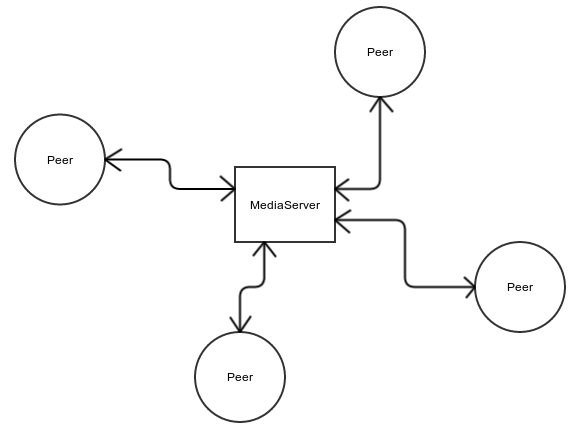
\includegraphics[scale=0.6]{mediaserver.png}
\\
\\
Communication between peers and the media server is done by opening up ports in the firewall to listen for incoming tcp and udp connections. The media server can receives incoming streams and mix it in with the other streams and forward it to all the other peers. All the streams are identified using an SSRC.

\subsubsection{Signaling}
Virtual Arena uses a proprietary way of doing signaling over RTCP.

\subsubsection{Transport}
Raw RTP stream over UDP.

\subsubsection{Media}
Speex for audio and theora for video.


\subsection{How does WebRTC work?}
WebRTC is a very complex synergy of components and protocols. But from a frontend developers point of view, all of this is packaged into three main Javascript API's: getUserMedia, RTCPeerConnection and RTCDataChannel. These are defined by the \gls{w3c}. 

The exchange of real-time media between two browsers follows a process like this:
\\
\\
1 Input devices are opened for capture as the media source. This is done using the getUserMedia API.
\\
\\
2 Now we have to signal the other users that we want to connect to them. using RTCPeerConnection we send an \gls{sdp} offer to the other clients, which generates an \gls{sdp} Answer.The \gls{sdp} here includes \gls{ice} candidates. Which opens ports in the firewall. There is a fallback if both clients are on symmetric \gls{nat}'s and a connection isn't possible to use a \gls{turn} server that acts like a packet mirror, channeling all the packets through the \gls{turn} server.
\\
\\
3 Once connection is successful, a \gls{dtls} connection is opened and all the media from input devices are encoded into packets and transmitted using \gls{srtp}-\gls{dtls} streams.
\\
\\
4 At the destination, the packets are decoded and formatted into a MediaStream.
\\
\\
5 The MediaStream is sent to output devices
\\
\\

\subsection{What are the differences?}
While Virtual Arena provides a very simple and not so secure solution media level. This because in a closed enterprised environemnt this is not needed. Most of the security will lie in the firewall anyways.

But since \gls{wrtc} is a very open solution and is supposed to work with public users firwall configurations, a lot more complex security architecture is needed.

So while \gls{wrtc} packages all their streams in a new format called a MediaStream. At the transport level everything is encrypted using \gls{dtls} on top of \gls{srtp}.

\subsection{What do we need?}
There are several problems here. Since Virtual Arena operates on a low-level not much is needed. All we need is to listen to a specific ip-address on a specific port on UDP transmitted data. In the packet headers we will find an \gls{ssrc} that we use to identify the incoming packets.

With WebRTC on the other hand, we are only allowed to work on a higher level. We cannot access MediaStreams directly without first opening a connection with another peer. This is a problem. This means that we first have to iniate a normal RTC Connection before we can look at any identifiers such as the \gls{ssrc}. We cannot listen on specific ports for incoming RTC connections, and we cannot specify a specific port to transmit data. Also as of now the current implementation of WebRTC is not designed to add local external streams to the connection. This means that getting WebRTC to work with any external application, we have create some sort of gateway server.
\\
\\
\textbf{By having done tons of experiments I propose this solution:}
\\
\\
One gateway server that can listen to UDP-packets from the Visual Solutions \gls{mcu} and acts as a peer in WebRTC. This is not an ideal approach, but the most viable at the moment. Ideally one would integrate WebRTC over the whole spectrum, which is both inconveniant and leads to complications.

For a single person that acts as a PeerConnection in WebRTC to listen in on a conversation from Virtual Arena, one would need to initiate a fake RTC Connection using two peers, then create a MediaStream from the incoming UDP packets and inject that MediaStream into the RTC Connection. On the returning side one would have to take the MediaStreams and break them into pure RTC packets with an SSRC identifier in the header and send them in return to the \gls{mcu}.

First problem is receiving the incoming conversation from Virtual Arena this can be done setting up a socket that listens for incoming UDP packets. This is not a problem and can even be done in a pure Javascript environment using node.js

Then one would have to create a MediaStream Object from these packets. This is not currently possibly using chrome API's or Firefox. In chrome it is possible to create a pure audio MediaStream using the new WebAudio API, and in Firefox it should be possible to create a MediaStream from video using getStreamUntilEnded(), but this is currently broken. In the future however this should be possible using the drafted captureMedia API.

It is however possible to inject external MediaStreams into an RTC Connection.

For returning data from a PeerConnection to the \gls{mcu} on would have to record the stream and return the data over a an \gls{udp} connection. This should be done using the proposed MediaStream Recording APIs, but none of the browser have currently implemented these yet.

\chapter{The Solution}
%!TEX root = ../main.tex


Enterprises and firewall
SBC and firewall traversal
Integration and interoperation

Necessary
Aims of the integration
Requirements


Suggestions about the integrated solution
Protcols
Network

Problems about the integrated solution


How can we integrate RTC in the Web with Virtual Arena?
There are two solutions to this problem the way I see it. The first is very obvious and complicated, but probably the best solution. The second is more of an experimental hack rather than a viable solution.

\section{The Gateway Solution}
The obvious solution is to create a gateway using \gls{wrtc} and Visual Arena to turn any \gls{wrtc} enabled browser into a client. The gateway will allow the web browser on your preferred device to make and receive connections from Virtual Arena. The gateway would have to contain three modules:
a Signaling Proxy, a Transport Proxy, and a Media Transcoder. The global architecture would look something like this:
\\
\\
\centerline{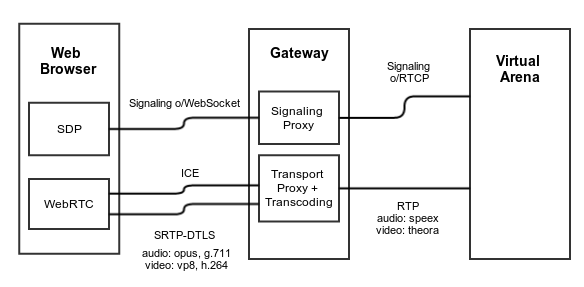
\includegraphics[scale=0.6]{gateway_architecture.png}}

\subsection{The Signaling Proxy}
Since \gls{wrtc} does not define any signaling protocol, one is free to use something custom made. But in this approach, the key information that needs to be exchanged is the \gls{sdp}, which specifies the necessary transport and media configuration information necessary to establish a connection. This approach is outlined by \gls{jsep}. So the role of the Signaling Proxy module would be to extend the custom signaling protocol already used in Virtual Arena to include the necessary metadata provided in the \gls{sdp}. It would go something lke this:

The \gls{mcu} sends an offer via the signaling method, then on the client the remote party would install it using the setRemoteDescription() API.

\begin{lstlisting}[frame=single]
...snip...
m=audio 1 RTP/SAVPF 111 103 104 0 8 106 105 13 126
c=IN IP4 0.0.0.0
a=rtcp:1 IN IP4 0.0.0.0
a=ice-ufrag:fAYfQM/iWMQPqiHs
a=ice-pwd:pgbuPPRdpKq+obC0lyRxVDe/
a=extmap:1 urn:ietf:params:rtp-hdrext:ssrc-audio-level
a=rtpmap:111 opus/48000/2
a=maxptime:60
a=ssrc:2209464108 cname:7oIEPieg3XZzHJdN
a=ssrc:2209464108 mslabel:uWu6kVvHhYbbkOtNalf5E2LFgjx4cpGMhnfo
a=ssrc:2209464108 label:2b626a18-c54c-4c1b-9f42-03519a9b63f2
m=video 1 RTP/SAVPF 100 116 117
...snip...
\end{lstlisting}

\subsection{The Transport Proxy}
The \gls{wrtc} specification make support for \gls{ice} and \gls{srtp}-{dtls} mandatory. The problem here is that Virtual Arena uses raw \gls{rtp} streams, it does not need the added security layers that \gls{wrtc} defines. It is up to the Transport Proxy to convert the media streams to allow these two worlds to interoperate. 

How can we take advantage of \gls{ice} and it's security? By modifying a constraint in the IceTransport object we can modify which candidates the ICE engine is allowed to use. We can indicate that the engine must use only relay candidates. This can be used to prevent leakage of IP addresses.


\subsection{The Media Transcoder}
The \gls{wrtc} specification defines these mandatory codecs:
\begin{itemize}
    \item Audio: opus and g.711
    \item Video: ?
\end{itemize}

There are still discussions on the topic of which video codec should be standard. The choice is between VP8 and H.264. The H.264 codec was recently made free by Cisco, so now both choices are royalty free. H.264 is the most widely deployed and currently has the best hardware support, but both Google and Firefox has decided to use VP8 in their WebRTC implementations.

Virtual Arena uses Speex for audio and Theora for video. So these would have to be transcoded to the appropriate formats.

This is one of the advantages of utilizing a \gls{mcu} because you can add support for both H.264 and VP8 and be able to create a session between  both Chrome, Virtual Arena, and Bowser.


\section{The Experimental Solution//TO DO}

%%EXPERIMENTAL SOLUTION%% EXTRA CHAPTER???
A server that acts like a client. This could be done using the native client library. One problem with the native library is that it as far behind the web APIs in terms of development. This is because all the focus is on browser-to-browser scenarios. There are a couple of services out there that uses the native libraries, but most are commerce. There is one open-source solution that has the ability to create a server that acts like client, but we need more than that. We need to be able to attach remote incoming RTP streams to a peer connection. Signaling is already done on the server side so that should not be any different from the previous solution. What we need is one gateway server that can listen to UDP-packets from Virtual Arena and act as a peer in \gls{wrtc}. This is not an ideal approach, but pretty cool if it should work.

For a single person that acts as a PeerConnection in WebRTC to listen in on a conversation from Virtual Arena, one would need to initiate a fake RTC Connection using two peers, then create a MediaStream from the incoming UDP packets and inject that MediaStream into the RTC Connection. On the returning side one would have to take the MediaStreams and break them into pure RTC packets with an SSRC identifier in the header and send them in return to the \gls{mcu}.

First problem is receiving the incoming conversation from Virtual Arena this can be done setting up a socket that listens for incoming UDP packets. This is not a problem and can even be done in a pure Javascript environment using node.js

Then one would have to create a MediaStream Object from these packets. This is not currently possibly using chrome API's or Firefox. In chrome it is possible to create a pure audio MediaStream using the new WebAudio API, and in Firefox it should be possible to create a MediaStream from video using getStreamUntilEnded(), but this is currently broken. In the future however this should be possible using the drafted captureMedia APIs.

It is however possible to inject external MediaStreams into an RTC Connection.

For returning data from a PeerConnection to the \gls{mcu} on would have to record the stream and return the data over a an \gls{udp} connection. This should be done using the proposed MediaStream Recording APIs, but none of the browser have currently implemented these yet.

%\chapter{How well does Real-time Communcation scale on mobile devices?}

\chapter{What will happen with the support of Real-time Communications in the near future?}

%\chapter{The Approach(experiments)}%

%\chapter{The Implementation(how implemented approach)}%

%\chapter{Evaluation}%

\chapter{Discussions and Conclusion}
%!TEX root = ../main.tex

summarize your thesis again as in the introduction.
Describe how your evaluation revealed that your system is successful.
Describe future work in this area.

We have looked at some basic theory about streaming media in the web browser, and explained our experiments and their capabilities. In chapter x we looked at the testing data collected and did an analysis of the results. The results were discussed and conclusions were made. This chapter will summarize the key elements of the results, look at what contributions have been made, and suggest some future work.


To simulate a low latency environment all early experiments were done on a local network. After collecting data using different mechanisms of protocols and streaming media, they were compared with the results from the same experiments using a simulated external network. Data about traffic, latency, and cpu-load were gathered and analyzed. Then we discussed the results with regard to inconsistencies, trends, synergies between different factors, and potential conclusions that could be made.

Contributions to reseach

Future Work
Furter testing when different vendors have agreed on a common platform



%research on rtcweb


By researching on the integration of RTCWEB technology with enterpirse communication systems can helkp business utilize RTCWEB to provide services through INternet or mobile Internet using their existing infrastructure in combination with a gateway. The can extend their services by reaching a ton of new devices. 
Through the research, we describe an integration solution by adding an interworking gateway which include three subsystems- singaling gateway, media relay and address server. Suggested protocols include WebSockets and RTP.
Aside from theory, this solution can realize the integration of RTCWeb with an enterprise communication system but the realization need th supporting of by standardization work like protocol and codec defining. IETF's standardization work is progreseed very quickly. In the the future, we will focus on the progressing and refine the solution. At the same time, realize a prototype.


% END SECTION %
\appendix
\chapter{Appendix Title}b
%% APPENDIX GOES HERE %%

\printglossaries

\bibliographystyle{plainnat}
\bibliography{Remote}

\end{document}